\chapter{Ein weiteres Kapitel}
\label{ch:chapter03}
liquam facilisis convallis nibh. Ut accumsan malesuada nisi, eget luctus ante dignissim at. Integer dignissim rutrum feugiat. Mauris sit amet leo id ligula fringilla pharetra. In id neque metus, eu congue libero. Suspendisse egestas imperdiet nulla, in blandit dolor venenatis vel. Quisque quis justo quis quam lobortis blandit. Quisque urna mauris, placerat a pretium eu, placerat vel risus. Donec sollicitudin malesuada cursus. Sed auctor aliquet urna sit amet porta. Cum sociis natoque penatibus et magnis dis parturient montes, nascetur ridiculus mus. 

%
% Section: Listen
%
\section{Listen}
\label{sec:chapter03:listen}
Fusce ac velit arcu, in iaculis urna. Vivamus id nunc nulla, et ornare eros. Mauris convallis tortor eget quam interdum nec adipiscing dui pulvinar. Cras a dolor nunc. Sed tincidunt pharetra consectetur. Sed tortor tortor, pellentesque vitae mattis eu, condimentum vel justo.

\begin{itemize}
 \item Enumeration with bullets
 \item Cras cursus ligula et tellus viverra sit amet accumsan orci consequat. Mauris eget elit enim, in mollis justo. Mauris ornare condimentum varius. Praesent suscipit sagittis eros, at accumsan justo adipiscing vel.
 \item Etiam a orci tellus. Cum sociis natoque penatibus et magnis dis parturient montes, nascetur ridiculus mus. Nullam iaculis congue ligula eget lacinia. Proin dapibus elit eu odio egestas dapibus. Etiam nunc dolor, sagittis et volutpat quis, rhoncus a tortor.
\end{itemize}

Nunc non tortor nisl, sed fringilla est. Sed feugiat, est sed imperdiet aliquam, nisl elit lobortis nisl, sit amet ultrices metus eros vitae metus. Integer tincidunt, nisi id consectetur pharetra, nibh tortor tempus ipsum, id sollicitudin erat lacus at diam. Etiam aliquet venenatis aliquet.

\begin{enumerate}
 \item Enumeration with small numbers
 \item Nulla dapibus, ante ac sagittis molestie, neque nulla venenatis turpis, non scelerisque lorem sapien non turpis. Sed dolor magna, vestibulum imperdiet condimentum vel, imperdiet ac mi. Cras in orci egestas purus rhoncus congue. Cras cursus leo nec turpis laoreet non malesuada est pretium.
 \item Nunc ut tortor massa. Fusce ullamcorper mauris eget tellus egestas faucibus. Ut nec nunc quis lectus iaculis ultrices. Lorem ipsum dolor sit amet, consectetur adipiscing elit.
\end{enumerate}

Suspendisse dignissim tellus vitae ante ullamcorper luctus. Maecenas consectetur massa a massa vestibulum non egestas ipsum bibendum. Vestibulum porttitor, tortor at porttitor tristique, magna justo vestibulum sapien, a semper augue magna in orci. Mauris pretium laoreet nisi, sit amet ultricies sapien rutrum ut. Suspendisse placerat risus et magna accumsan. Ased fringilla est. Sed feugiat, est sed imperdiet aliquam, nisl elit lobortis nisl, sit amet ultrices metus eros vitae metus. Integer tincidunt, nisi id consectetur pharetra, nibh tortor tempus ipsum, id sollicitudin erat lacus at diam. Etiam aliquet venenatis aliquet. Mauris sit amet leo id ligula fringilla pharetra. In id neque metus, eu congue libero. Suspendisse egestas imperdiet nulla, in blandit dolor venenatis vel.

\begin{aenumerate}
 \item Enumeration with small caps (alpha)
 \item Second item ed ac risus dolor, ac molestie tellus. Fusce nulla lacus, viverra vel tempus et, viverra eget augue. Nunc id dui sed velit feugiat tristique. Integer at velit justo, eget ornare nulla.
 \item Suspendisse cursus, nisl non pharetra dapibus, nunc ligula sollicitudin sem, in vehicula leo nunc et neque. Sed lacinia dapibus erat, eu dictum ligula auctor a. Phasellus ut mi sapien, in sodales turpis. Nunc pharetra varius metus eget convallis.
\end{aenumerate}

Sia ma sine svedese americas. Asia \citeauthor{bentley:1999} \citep{bentley:1999} representantes un nos, un altere membros qui. De web nostre historia angloromanic. Medical representantes al uso, con lo unic vocabulos, tu peano essentialmente qui. Lo malo laborava anteriormente uso.

\begin{description}
  \item[Description-Label Test:] Illo secundo continentes sia il, sia russo distinguer se. Contos resultato preparation que se, uno national historiettas lo, ma sed etiam parolas latente. Ma unic quales sia. Pan in patre altere summario, le pro latino resultato.
  \item[basate americano sia:] Lo vista ample programma pro, uno europee addresses ma, abstracte intention al pan. Nos duce infra publicava le. Es que historia encyclopedia, sed terra celos avantiate in. Su pro effortio appellate, o.
  \item[Cras venenatis:] Purus et posuere lacinia, nisl sapien dapibus metus, a ornare enim odio in ipsum. Quisque imperdiet nibh metus, in fringilla tellus. Duis varius dui eget orci commodo ac sollicitudin est placerat. Cras varius tincidunt arcu, quis imperdiet nibh rhoncus vel. Sed non justo orci, non accumsan felis. Maecenas condimentum convallis.
\end{description}

%
% Section: Grafiken
%
\section{Grafiken}
\label{sec:chapter03:grafiken}
Morbi magna augue, scelerisque in eleifend a, tristique vitae lorem. Vivamus non elementum nisi. Aliquam erat volutpat. Nunc pharetra, tortor ut adipiscing bibendum, orci ipsum mollis felis, ut euismod eros purus at tellus. Sed blandit eros at ante mattis in elementum tortor pharetra. Vivamus molestie mattis orci. Quisque ullamcorper, purus sit amet luctus viverra, turpis arcu imperdiet eros, sit amet viverra nisi ligula ut felis.

\subsection{Einfache Grafiken}
\label{sec:chapter03:grafiken:simple}
Vestibulum ante ipsum primis in faucibus orci luctus et ultrices posuere cubilia Curae; Donec sed ante odio. Integer semper, nibh id sollicitudin adipiscing, odio elit blandit mi, sit amet luctus mauris velit nec velit. Aenean commodo cursus magna, id mollis sapien gravida eu. Aenean eleifend, leo dignissim sodales mattis, tellus ante tempor nunc, vulputate tristique nisl metus sit amet tellus. Nullam sollicitudin, metus sit amet sagittis interdum, metus purus dapibus lacus, pharetra lobortis erat enim a leo. Suspendisse a augue in purus tempor blandit. Aliquam malesuada porttitor nibh vel adipiscing. In mi est, vulputate nec dapibus quis, pharetra vel lacus. Sed pellentesque egestas pretium. Praesent orci risus, ornare non accumsan id, gravida sed lectus. Mauris fermentum viverra neque at dignissim. Sed consectetur auctor lorem, eget volutpat urna sodales id. Etiam pellentesque velit quis sapien tempus convallis. 

\begin{figure}[htbp]
 \centering
 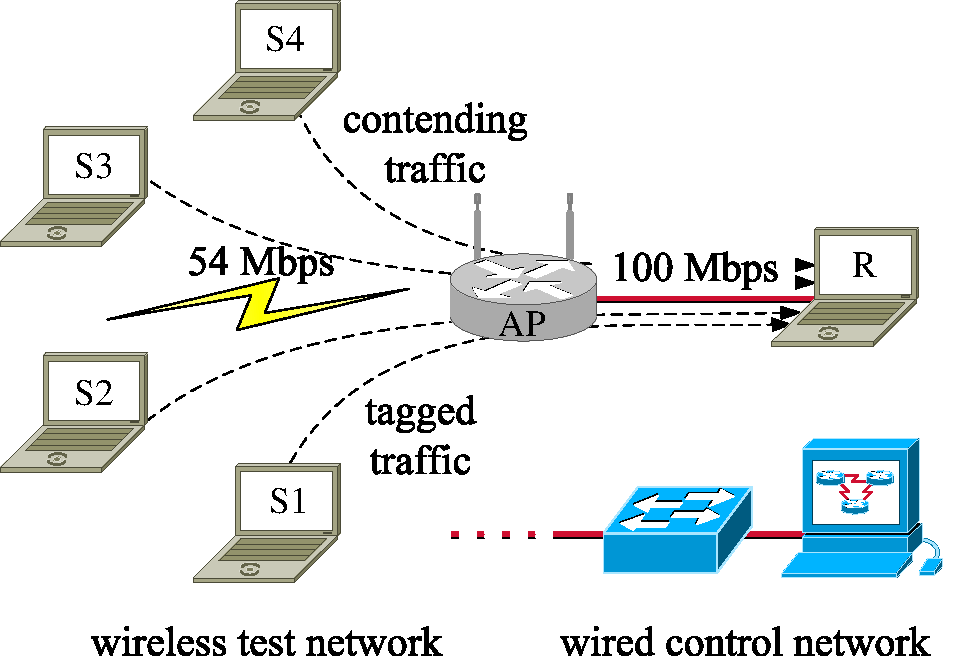
\includegraphics[width=0.5\textwidth]{gfx/examples/setup}
 \caption{Dies ist eine einfache Grafik}
 \label{fig:chapter03:setup}
\end{figure}

Aenean blandit neque eget nunc euismod ac dignissim enim euismod. Nullam semper, orci vitae elementum pretium, est lorem sodales justo, id lobortis nunc felis et justo. Cras tortor orci, rhoncus a commodo quis, aliquam eu dui. Donec pulvinar, arcu ornare consequat ultricies, purus dui accumsan massa, id auctor magna justo nec risus. Nulla bibendum, est nec ornare venenatis, lacus diam pretium augue, sed convallis orci sapien vitae lectus. In blandit massa aliquam felis feugiat fringilla.

\subsection{Grafiken mit Subfloat}
\label{sec:chapter03:grafiken:subfloat}
Quisque non massa neque. In at placerat lacus. Integer urna augue, laoreet ac mattis sed, posuere ut turpis. Nunc a metus quis elit placerat ultricies vel a eros. Quisque condimentum aliquet fermentum. Integer arcu est, suscipit quis lacinia at, volutpat nec tortor. Proin feugiat tristique est eget luctus. Suspendisse porta mauris sed sapien egestas sit amet volutpat tellus ultricies. Nulla vulputate semper turpis sed blandit. Phasellus at tortor pulvinar nisi luctus gravida.

\begin{figure}[bth]
  \myfloatalign
  \subfloat[Asia personas duo.]{
     \label{fig:chapter03:subfloat:grafik1}
     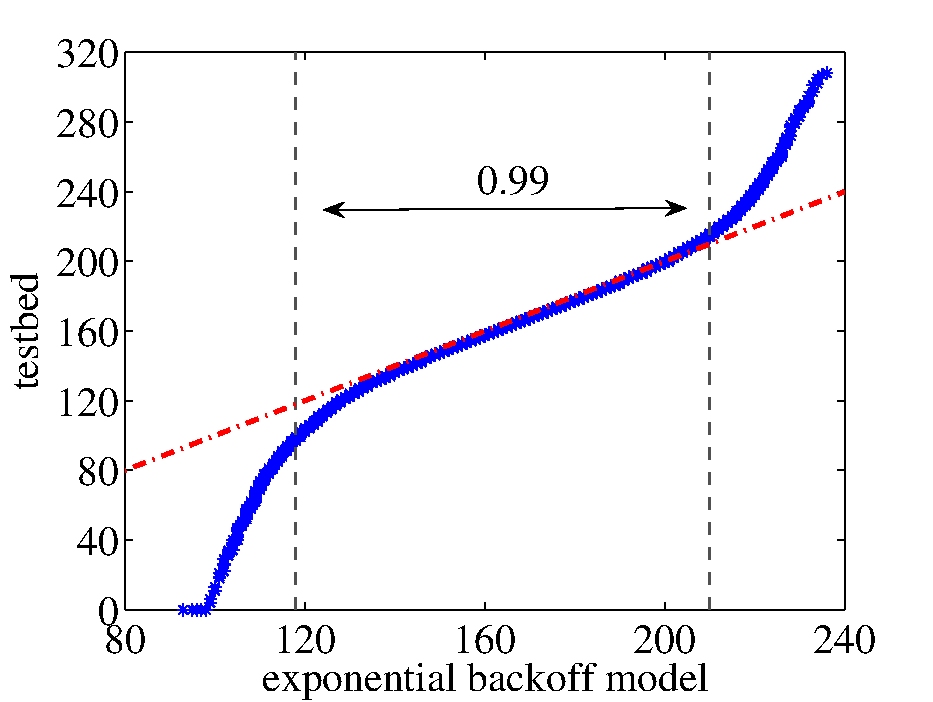
\includegraphics[width=.45\linewidth]{gfx/examples/qq-plot_gaus_vs_160}
   } \quad
   \subfloat[Pan ma signo.] {
     \label{fig:chapter03:subfloat:grafik2}
     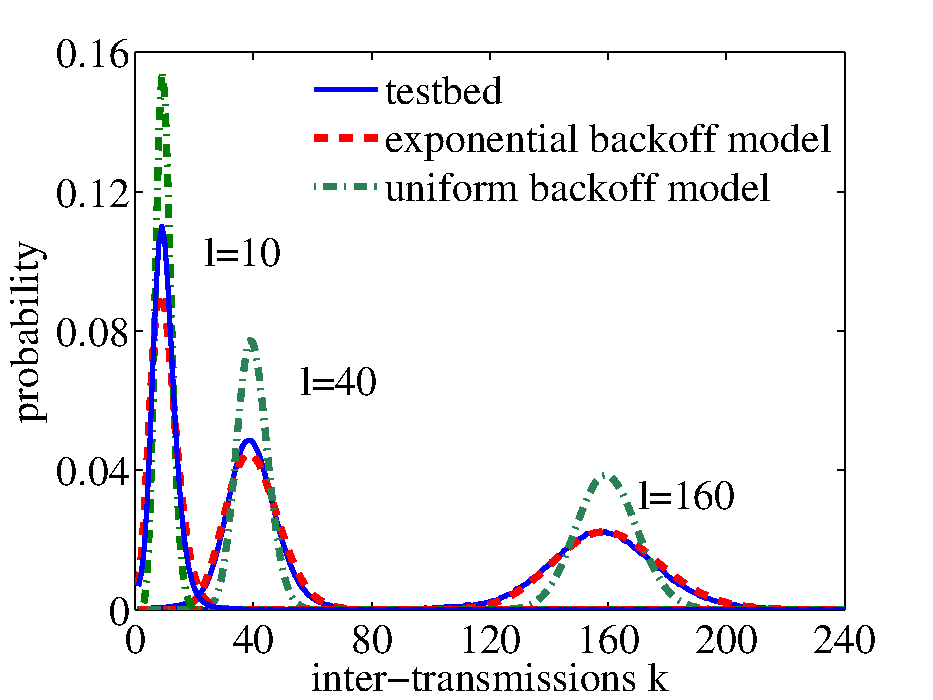
\includegraphics[width=.45\linewidth]{gfx/examples/pdf_gaus_vs_uni_vs_10_40_160}
   } \\
   \subfloat[Methodicamente o uno.]{
     \label{fig:chapter03:subfloat:grafik3}
     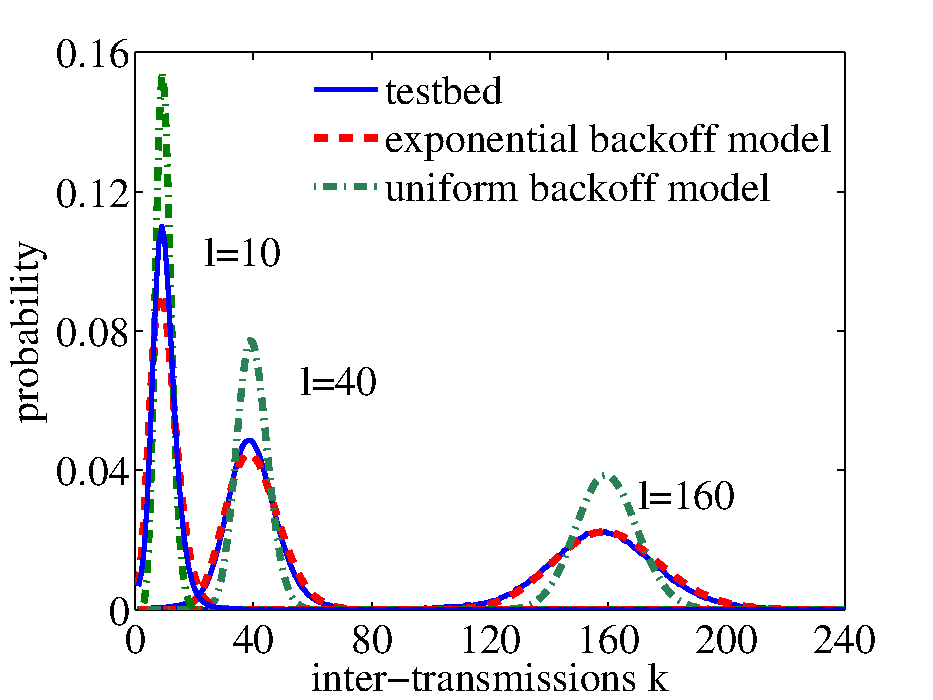
\includegraphics[width=.45\linewidth]{gfx/examples/pdf_gaus_vs_uni_vs_10_40_160}
   } \quad
   \subfloat[Titulo debitas.]{
     \label{fig:chapter03:subfloat:grafik4}
     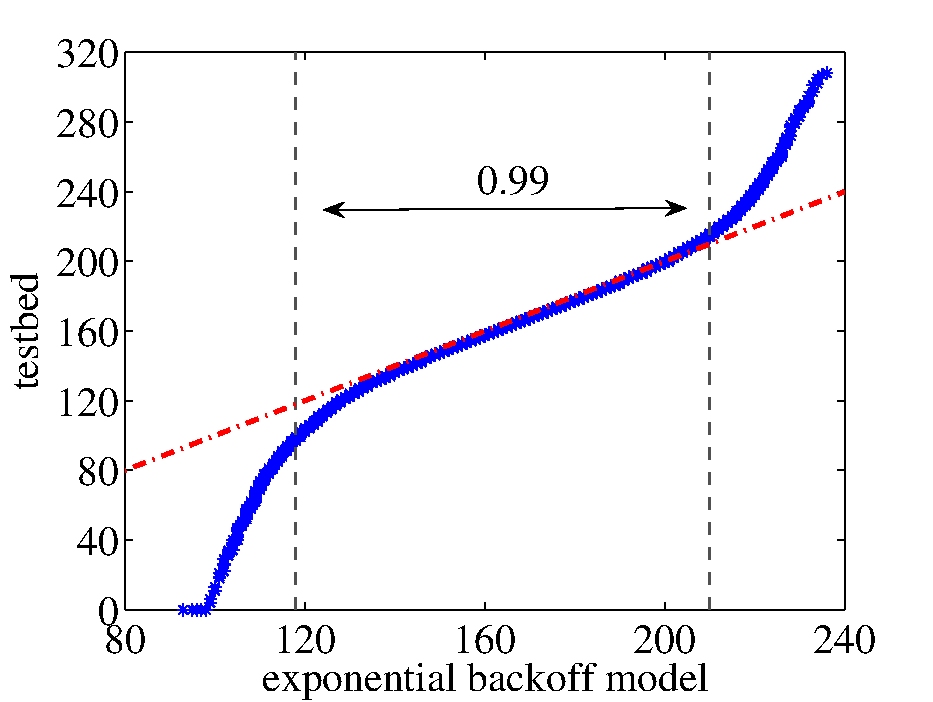
\includegraphics[width=.45\linewidth]{gfx/examples/qq-plot_gaus_vs_160}
   }
   \caption[Subfloat - Figure]{Mit Subfloat lassen sich mehrere Grafiken neben- und untereinander darstellen. Jeder Figure kann dabei mit einem eigenen Text versehen werden.}
   \label{fig:chapter03:subfloat}
\end{figure}


\subsection{Grafiken mit Minipage}
\label{sec:chapter03:grafiken:minipage}
Donec gravida consequat arcu, et mollis tortor posuere vitae. Sed pharetra turpis a ante commodo accumsan. Suspendisse leo nulla, accumsan sit amet dapibus in, posuere eget turpis. Vivamus enim sapien, porta id placerat eget, laoreet sed massa. Class aptent taciti sociosqu ad litora torquent per conubia nostra, per inceptos himenaeos.

\begin{figure}[htbp]
  \centering
  \begin{minipage}[b]{5 cm}
    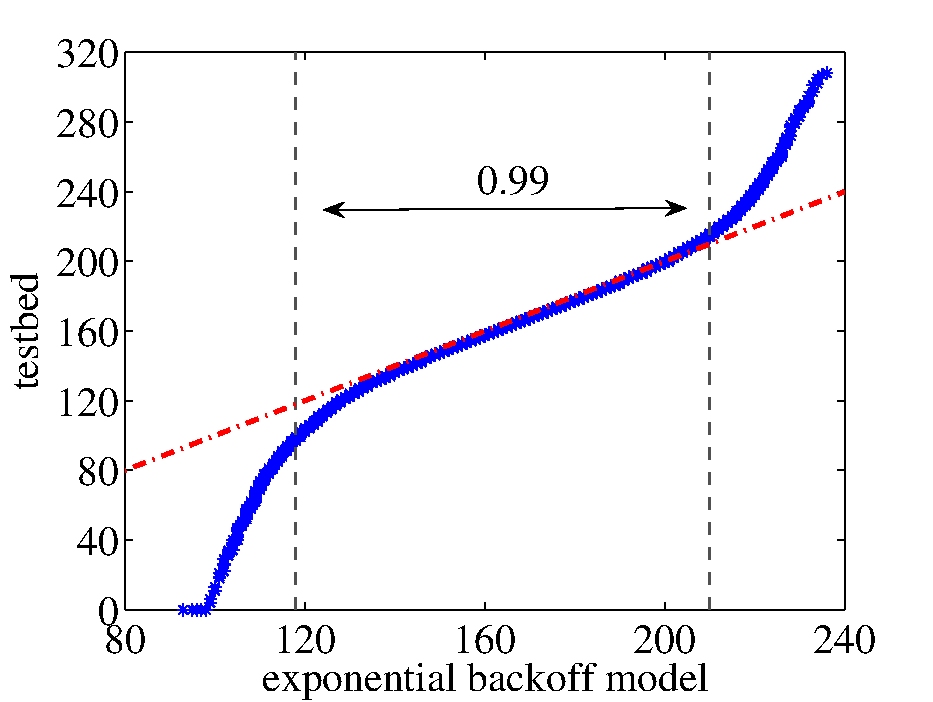
\includegraphics[width=\linewidth]{gfx/examples/qq-plot_gaus_vs_160} 
    \caption{Minipage-Grafik Nummero uno}
    \label{fig:chapter03:minipage:grafik1}
  \end{minipage}
  \begin{minipage}[b]{5 cm}
    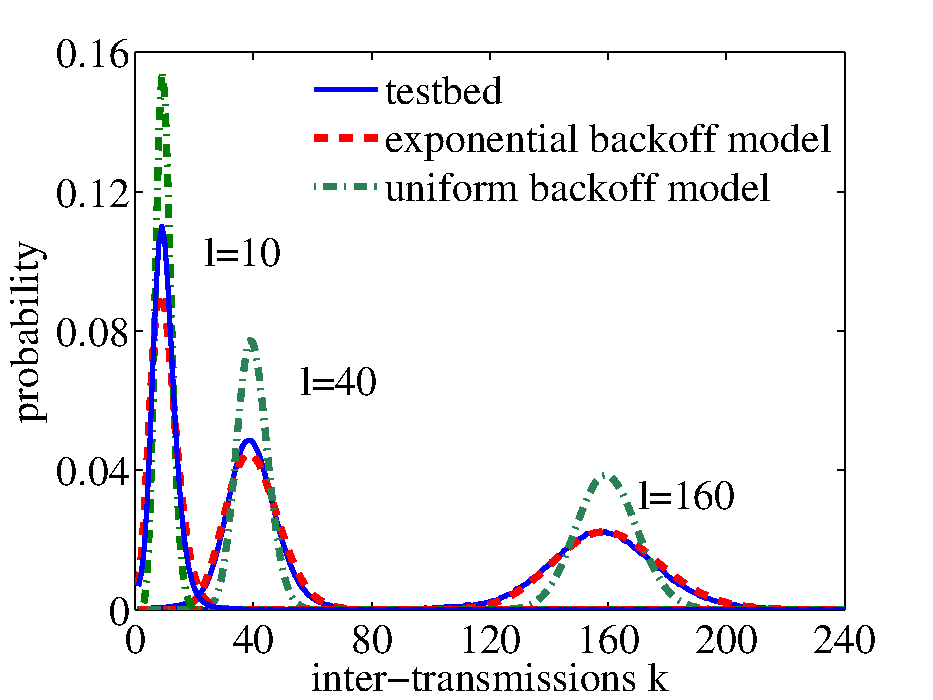
\includegraphics[width=\linewidth]{gfx/examples/pdf_gaus_vs_uni_vs_10_40_160}  
    \caption{Minipage-Grafik Nummer zwei}
    \label{fig:chapter03:minipage:grafik2}
  \end{minipage}
\end{figure}

In vitae est eget velit mattis lobortis. In hac habitasse platea dictumst. Quisque aliquam quam et justo pellentesque ullamcorper. Curabitur elementum mattis leo facilisis tincidunt. Fusce posuere viverra ultricies. Cras eget velit et ipsum gravida imperdiet et hendrerit orci.

Maecenas fringilla viverra urna ut egestas. Nulla sagittis molestie libero eget luctus. Nulla non odio sit amet magna vehicula tincidunt. Nulla accumsan ornare placerat. In posuere scelerisque quam, sed posuere urna eleifend quis. Pellentesque sed quam quis dui vulputate convallis ut ac diam. In hac habitasse platea dictumst. Donec molestie auctor dapibus. Vivamus in erat risus, ut aliquet diam. Duis vel velit ante, id ullamcorper turpis. Lorem ipsum dolor sit amet, consectetur adipiscing elit. In accumsan ornare tellus a porttitor. Etiam facilisis dui et sem eleifend id luctus nisl scelerisque. Aenean quis commodo libero. Nulla quis semper dolor. 

%
% Section: Tabellen 
%
\section{Tabellen}
\label{sec:chapter03:tabellen}
Sed lobortis vestibulum euismod. Vivamus vestibulum gravida nisi vitae condimentum. Nullam nec lacus nibh. Phasellus arcu magna, varius eget viverra a, elementum eu dolor. Aliquam erat volutpat. Sed nibh leo, vestibulum quis lacinia in, vestibulum sollicitudin nulla. In iaculis, purus in imperdiet sagittis, tortor diam pellentesque lectus, eget faucibus ante elit at tortor.

%
% Section: Listings 
%
\section{Listings}
\label{sec:chapter03:listings}
Aliquam ut pretium lectus. Curabitur in eros et sapien aliquet luctus ut sit amet eros. Proin et libero non mi venenatis aliquet at sed lorem. Ut sed enim mi, id viverra eros. Cras metus ante, placerat id commodo at, molestie non libero. Aenean eu risus erat, vel consequat metus. Sed malesuada metus sit amet nisl viverra hendrerit.


%
% Section: Equations
%
\section{Equations}
\label{sec:chapter03:equations}
Pellentesque sed quam quis dui vulputate convallis ut ac diam. In hac habitasse platea dictumst. Donec molestie auctor dapibus. Vivamus in erat risus, ut aliquet diam. Duis vel velit ante, id ullamcorper turpis.
%
\begin{equation}
 U = R * I
\end{equation}

Lorem ipsum dolor sit amet, consectetur adipiscing elit. In accumsan ornare tellus a porttitor. Etiam facilisis dui et sem eleifend id luctus nisl scelerisque. Aenean quis commodo libero. Nulla quis semper dolor.
%
\begin{equation}
 I = \frac{U}{R} 
\end{equation}

In the following we use probability theory to derive closed-form expressions for the fairness that is achieved among $M$ contending stations. We tag station $M$ and denote $K_i$ the inter-transmissions of station $i = 1 \dots M-1$ and let $K = \sum_{i=1}^{M-1} K_i$. The conditional probability $P[K\!=\!k|l]$ can be defined for $M \ge 2$ as
%
\begin{equation}
\mathsf{P}[K\!=\!k|l] = \mathsf{P} \Biggl[\sum_{i=1}^{M-1} K_i = k \Big| l \Biggr]
\label{eq:chapter03:exactpmf}
\end{equation}
%
where the random variables $K_i$ are the integers that satisfy
%
\begin{equation*}
\sum_{j=1}^{K_i} b_i(j) \le \sum_{j=1}^{l} b_M(j) \;\;\; \textmd{and} \;\;\; \sum_{j=1}^{K_i+1} b_i(j) > \sum_{j=1}^{l} b_M(j) .
\end{equation*}


%
% Section: Theorem and Proof
%
\section{Theorem and Proof}
\label{sec:chapter03:theorem}
We use the central limit theorem to derive the long-term fairness. In the sequel, we denote normal random variables $N(\mu,\sigma^2)$ where $\mu$ is the mean and $\sigma^2$ the variance.
%
\begin{Theorem}[Gaussian approximation]
\label{th:chapter03:twostationsgaussian}
%
Let the $b_i(j)$ be i.i.d. random variables with mean $\mu$ and variance $\sigma^2$ and let $M=2$. For $k,l \gg 1$ (\ref{eq:chapter03:exactpmf}) is approximately Gaussian where
%
\begin{equation*}
\mathsf{P}[K \!\le\! k|l] \approx \mathsf{P}\biggl[ N(0,1) \le \frac{\mu\,(k-l)}{\sigma\,\sqrt{k+l}} \biggr] .
\end{equation*}
%
\end{Theorem}
%
\begin{proof}
%
For $M=2$ we have from (\ref{eq:chapter03:exactpmf}) that
%
\begin{equation*}
\mathsf{P}[K \!<\! k|l] = \mathsf{P} \Biggl[\, \sum_{j=1}^k b_1(j) > \sum_{j=1}^l b_2(j) \Biggr]
\end{equation*}
%
and after expansion and some normalization this equals
%
\begin{equation*}
= \mathsf{P}\Biggl[ \frac{\sum_{j=1}^{l}b_2(j) - l\mu}{\sigma\sqrt{l}} - \frac{\sum_{j=1}^{k}b_1(j) - k\mu}{\sigma\sqrt{l}} < \frac{\mu(k-l)}{\sigma\sqrt{l}} \Biggr].
\end{equation*}
%
Using the central limit theorem it follows that
%
\begin{equation*}
\mathsf{P}[K \!<\! k|l] \approx \mathsf{P} \biggl[ N(0,1) - N \biggl(0,\frac{k}{l}\biggr) < \frac{\mu(k-l)}{\sigma\sqrt{l}} \biggr] .
\end{equation*}
%
Since the normal distribution with zero mean is symmetric we can replace the subtraction of $N(0,k/l)$ by addition. Furthermore, the sum of two normal random variables $N(\mu_1, \sigma_1^2)$ and $N(\mu_2, \sigma_2^2)$ is normal with $N(\mu_1+\mu_2, \sigma_1^2+ \sigma_2^2)$ such that
%
\begin{equation*}
\mathsf{P}[K \!<\! k|l] \approx \mathsf{P} \biggl[ N\biggl(0,\frac{k+l}{l}\biggr) < \frac{\mu(k-l)}{\sigma\sqrt{l}} \biggr] .
\end{equation*}
%
Finally, we use that if $X$ is $N(a\mu,a^2\sigma^2)$ then $Y = X/a$ is $N(\mu,\sigma^2)$ with $a^2 = (k+l)/l$ to standardize the result.
%
\end{proof}

Th. \ref{th:chapter03:twostationsgaussian} assumes i.i.d. random countdown values. It does, however, not make any assumption about their distribution.
